\documentclass[a4paper, 12pt, Ariel]{article}

\usepackage[english]{babel}
\usepackage[utf8]{inputenc}
\usepackage{amsmath}
\usepackage{graphicx}
\usepackage[colorinlistoftodos]{todonotes}
\usepackage{gensymb}
\usepackage{url}
\usepackage[a4paper, total={6in, 8in}]{geometry}
\usepackage{upgreek}
\usepackage{setspace}
\usepackage{caption}
\usepackage{subcaption}
\usepackage{float}
\usepackage{setspace}
\onehalfspacing


\begin{document}
\begin{titlepage}
   \begin{center}
       \vspace*{1cm}
 
       \bf{Autonomous Surface Vehicles (ASVs) equipped with broadband echosounders as survey platforms for an undisturbed epipelagic layer in the Arctic}
 
        
 
       \vspace{1cm}
 
       \textbf{Muriel Dunn}\\
       \text{Ph.D. Student in Fisheries Sciences}\\

 
       \vfill
 
       Research Proposal\\
	\today

 
       \vspace{2.9cm}
 
       %\includegraphics[width=0.4\textwidth]{university}
 
       Fisheries and Marine Institute\\
       Memorial University of Newfoundland\\
       St-John's, Newfoundland\\

	\vspace{0.5cm}

	Akvaplan-niva\\
	Tromsø, Norway\\

 
   \end{center}
\end{titlepage}


\tableofcontents

\newpage

\section{Introduction}
 It is widely understood that Arctic ecosystems are rapidly changing. The ecosystem changes are a response to physical changes such as warming waters and earlier ice breakup. Scientists and researchers rely on boat surveys to quantify the changes which help understand the ecosystem responses to the physical oceanographic and atmospheric trends. Boat surveys are expensive, primarily because of boat costs. The cost of boat surveys only increases for remote regions like the Arctic, because of the need for ice-strengthened vessels and the logistical challenges. However, it is also becoming increasingly important to monitor and research the Arctic as ice melt is opening up new areas for oil exploration and fishing.\\
 
\subsection{Arctic Acoustic Surveys}
The rapid changes in the Arctic and the high cost of traditional survey methods have introduced a need for alternative effective Arctic monitoring systems. Recent scientific and technological developments in ocean monitoring have advanced the field of ecosystem research by increasing the spatial and temporal coverage through hull-mounted acoustic-trawl surveys. Technology advances such as satellite, underwater gliders and surface moorings provide long term and autonomous data collection in regions that have historically been difficult or impossible to access. Significant advancements in technology are happening very quickly, but we must also process the data effectively for better ecosystem assessment tools \cite{Cross2015}.\\

\subsection{Sailbuoys equipped with broadband echosounders}
Further technology developments have lead to Autonomous Surface Vehicles (ASVs) for better monitoring of the epipelagic layer (0 - 100 m depth). Sailbuoys equipped with broadband echosounders represent new survey platforms that are non-invasive and, increase the duration and footprint of surveys. Sailbuoys are wind- and solar-powered ASVs that travel between prescribed waypoints. Broadband echosounders are sonars that use a wider bandwidth than narrowband echosounder, the industry standard. The wider bandwidth returns a measure of backscatter across a range of frequencies, which offers potential for discrimination and characterization of targets (i.e. fish or zooplankton and potentially to the species level). \\

The rapid changes, early ice breakup, reduced ice coverage and overall thinning of historical ice, have direct impacts on bloom timing of primary production which in turn effects the survivability of secondary producers \cite{Ringuette2002}. Primary and secondary producers aggregate in the few meters below the surface of the ocean during spring and summer \cite{Basedow2016}. However, conventional survey methods do not detect them because they are unable to measure the top of the water column. Conventional survey methods do not measure the top of the water column because the acoustic blind zone, the depth at which data collection begins, can reach 13 m with a hull-mounted sonar. For broadband echosounders on a Sailbuoy, the acoustic blind zone is reduced to 2 m because the echosounder is positioned directly below the surface. The reduced blind zone of this innovative survey platform enables documentating the abundance, spatial and vertical distributions of fish and zooplankton within the top meters of the water column. The top few meters below the surface is where primary and secondary producers as well as fish larvae aggregate, in the summer, during the ice free season which coincides with when research vessels can do ecological surveying . \\

Fish within the epipelagic layer (0 - 100 m) react to light from research vessels \cite{Ludvigsen2018} and vessel noise, even when using noise-reducing state-of-the-art research vessels \cite{Ona2007}, resulting in deeper and fewer fish detections \cite{DeRobertis2019}. For acoustic surveys in the Arctic, artificial light emitted from vessels can reduce (or increase) the measured backscatter due to the effect of artificial light on the behaviour of marine fish and zooplankton down to at least 200 m \cite{Berge2020}. Sailbuoys emit very little light and noise. They are a surveying platform that can monitor an undisturbed epipelagic layer. \\

 


\section{Barents Sea: A physical perspective}
The Barents Sea is a highly seasonal shelf sea that is part of the Arctic Continental shelf. The Barents Sea is positioned between the Greenland Sea and Kara Sea, north of continental Norway and Russia. It is a relatively shallow basin (230 m depth on average) that includes Spitsbergen, Franz Josef Land and Novaya Zemlya. The west side of the Barents Sea is restricted by the West Spitsbergen current, which runs along the west side of Spitsbergen and Franz Josef Land. On the west of the West Spitsbergen current is the Fram Strait. The Barents Sea and the Fram Strait supply Atlantic Water and some Arctic Intermediate Water into the Arctic Ocean \cite{Rudels1994}.

\subsection{Circulation}
The Barents Sea circulation pattern drives water mass transformations in certain areas of the shelf sea. There are four main water masses in the Barents Sea: Atlantic Water, Norwegian Coastal Current Water, Arctic Water and the Barents Sea Water. The southwestern section of the sea is composed of Atlantic Water; it originates from the Norwegian Atlantic current that runs up the coast of Norway and enters through the Barents Sea Opening, a trench also called Bjørnøyrenna, between Bjørnøya and continental Norway \cite{Ingvaldsen2002}, as indicated in Figure \ref{fig:currentsmap}. Atlantic Water is a warm and salty (\textgreater 35 PSU, \textgreater 3 \degree C) water mass that dominates the southwestern area of the Barents Sea \cite{Sakshaug2009}, red arrows in Figure \ref{fig:currentsmap}. \\

\begin{figure}[H]
	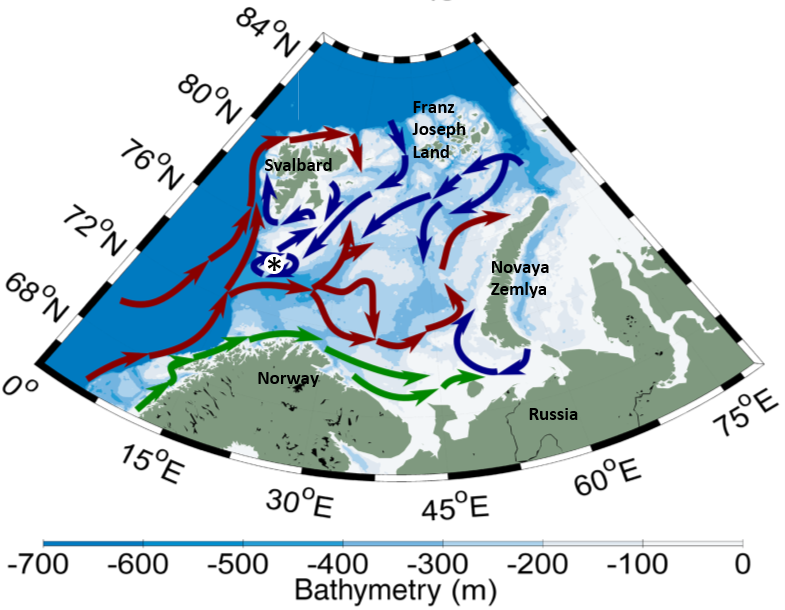
\includegraphics[width=\textwidth]{CurrentsMap.png}
	\centering
	\caption{A map of the Barents Sea with bathymetry. Red arrows indicate the circulation of warm and salty Atlantic water. Blue arrows indicate the circulation patterns from the cold and less saline Arctic Water. The small island Bjørnøya is marked by the star (*). Adapted from \cite{Oziel2016}}
	\label{fig:currentsmap}
\end{figure}


The Norwegian Coastal Current Water stays along the edge of the continent and has a wide range of temperatures throughout its vertical profile. The river runoff contributes to the strong stratification of the Norwegian Coastal Current Water. Overall it is slightly less salty (\textless 34.7 PSU) than the Atlantic Water. The Norwegian Coastal Current circulation is shown in Figure \ref{fig:currentsmap} as the green arrows following the continental coast of  Norway.\\

The Arctic Water dominates the northeastern part of the Barents Sea, it has low salinity (34.3 to 34.8 PSU) and is very cold (\textless 0 \degree C). Arctic Water enters the Barents Sea on both sides of Franz Joseph Land, as shown in Figure \ref{fig:currentsmap} as blue arrows. It is ice-covered in the winter and has a layer of meltwater at the surface in the summer which hinders mixing and increases stratification throughout the whole water column \cite{Sakshaug2009}.  \\

\begin{figure}[H]
	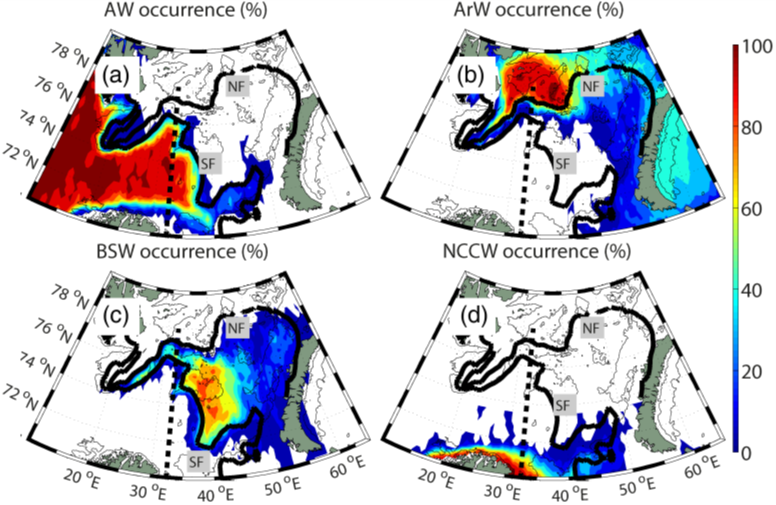
\includegraphics[width=\textwidth]{OzielWaterMass.png}
	\caption{Water mass in the 50 - 100 m layer across the Barents Sea in August-September between 1980-2011. In all panels, the polar front (black line) starts as a single line in the west, and after Bjørnøya it is split into Northern Front (NF) and Southern Front (SF). The panels show occurrences (\%) of a) Atlantic Water, b) Arctic Water, c) Barents Sea Water and d) Norwegian Current Coastal Water. Image from \cite{Oziel2016}.}
	\label{fig:polarfront}
\end{figure}


At the boundary between the warm and salty Atlantic Water and the cold and less saline Arctic Water is the polar front. In the western Barents Sea it is agreed that the polar front is constrained by topographic steering and follows the southern flank of Spitsbergenbanken (Figure \ref{fig:iceextent}). The isobath that contrains the polar front can vary from 50-m to 260-m \cite{Parsons1996, Vaage2014, Oziel2016}. The Sentralbanken (Figure \ref{fig:iceextent}) acts as a barrier for Atlantic Water across the polar front. The Sentralbanken seamount is a barrier because of well-mixed locally produced Polar Front Water in the Taylor column above the seamount \cite{Reigstad2002}. A Taylor column is an eddy trapped above an isolated seamount; it forms in a uniformly rotating fluid to conserve potential vorticity \cite{Chapman1992}. The broad range of isobaths might be due to a double front system: a shallower density front between the Arctic Water and the Polar Front Water and a potential vorticity front creating the topographic steering between the Polar Front Water and the Atlantic Water \cite{Hop2020}.\\

The eastern part of the polar front can be more dynamic. It is common to use strong coinciding gradients of temperature and salinity to describes the frontal structure in the west \cite{Skjoldal1987}. For the eastern Barents Sea, they find it is composed of two areas, the Northern polar front associated with the salinity gradient and the Southern polar front associated with the temperature gradient \cite{Oziel2016} (Figure \ref{fig:polarfront}). Between the Northern and Southern polar front, the Atlantic Water and Arctic Water form a dense brine when they are mixed during ice formation \cite{Pfirman1994}. The brine sinks and produces Barents Sea Water, which is convected to the Arctic and becomes Arctic Intermediate Water \cite{Rudels1994}, Figure \ref{fig:polarfront}c). Barents Sea Water contributes in part to the overturning circulation of the North Atlantic Ocean \cite{Oziel2016}. Changes in Barents Sea Water formation and properties due to variability in the climate will impact its contribution to the Arctic Intermediate Water and the overturning circulation of the North Atlantic Ocean.\\


\begin{figure}[H]
	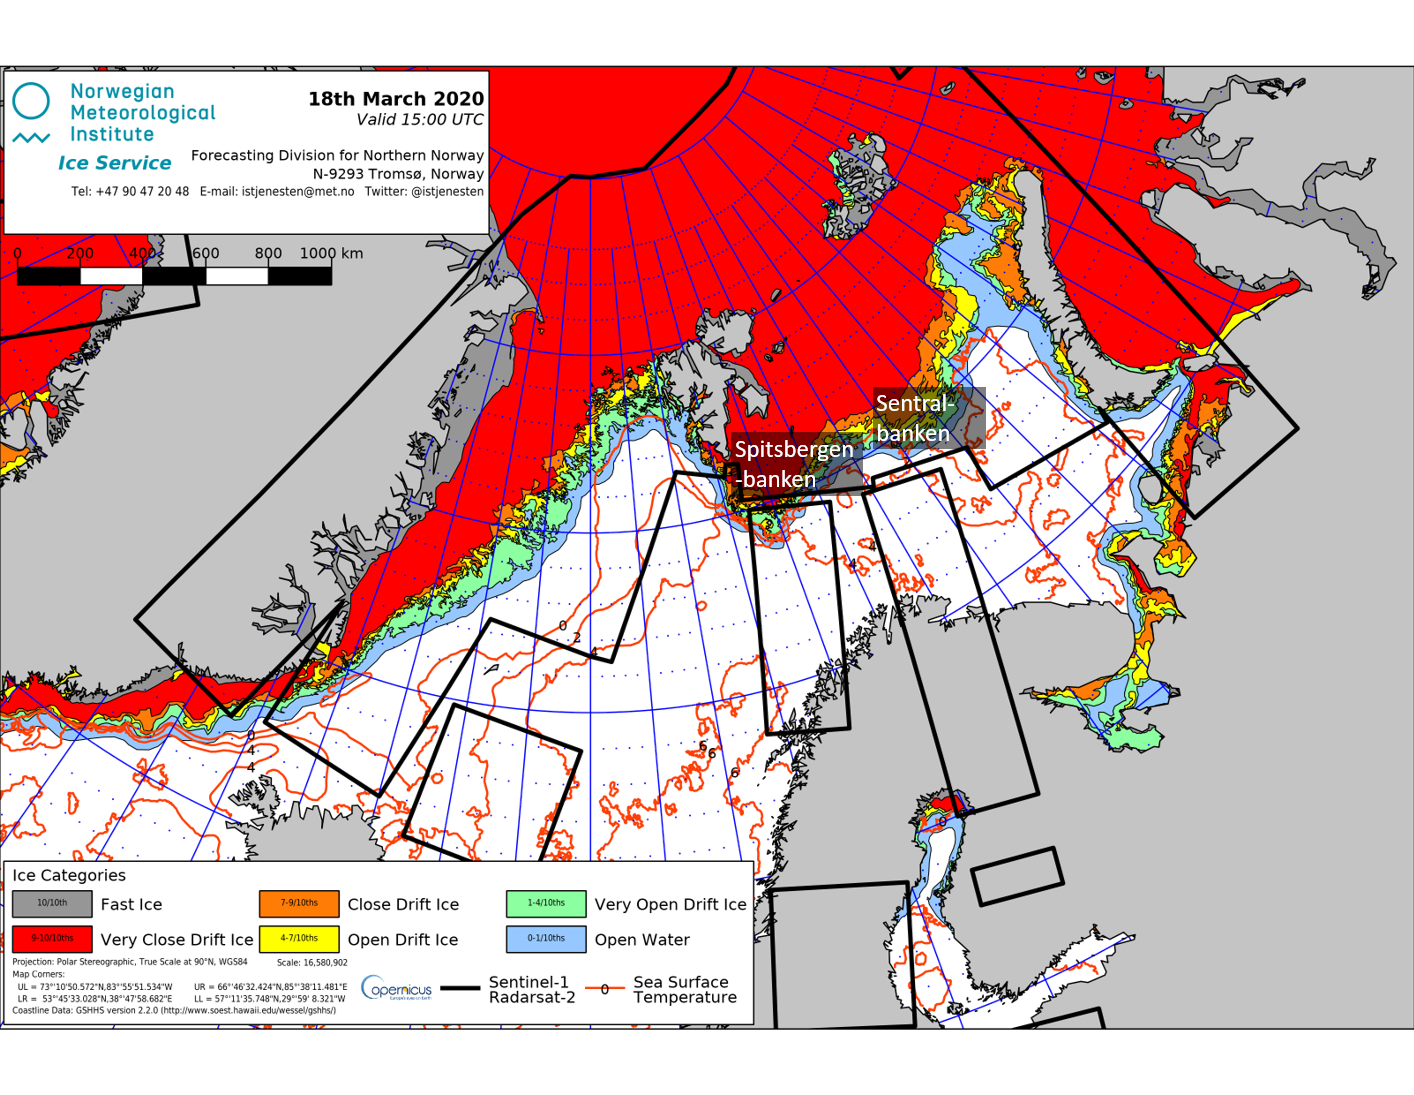
\includegraphics[width=\textwidth]{IceExtent18032020.png}
	\caption{Map of the Barents Sea ice extent on March 18th, 2020. Downloaded from the Norwegian Meterological Institute at www.cryo.met.no/en/latest-ice-charts.}
	\label{fig:iceextent}
\end{figure}

\subsection{Climate}
The Barents Sea climate has two positive feedback loop states: warm and cold. In some years, the warm periods can be correlated with a positive North Atlantic Oscillation (NAO) index. The NAO index describes the atmospheric pressure at sea-level between the subtropical high and the subpolar low. The pressure difference affects the direction and strength of the westerly winds. The NAO index is associated with weather and precipitation patterns in western and central Europe and eastern North America. In the Barents Sea, a positive NAO is indicative of strong southwesterly winds at the entrance of AW into the Barents Sea. The southwesterly winds increase the Atlantic Water inflow, which increases the temperature of the sea. The increase in temperature and Atlantic Water moves the polar front northwards and reduces the sea ice extent. The decreased sea ice extent increases the atmosphere/ocean heat flux, which creates low air pressure. The local low brings southwesterly winds and the positive feedback cycle repeats as shown in Figure \ref{fig:feedback}.\\

\begin{figure}[H]
	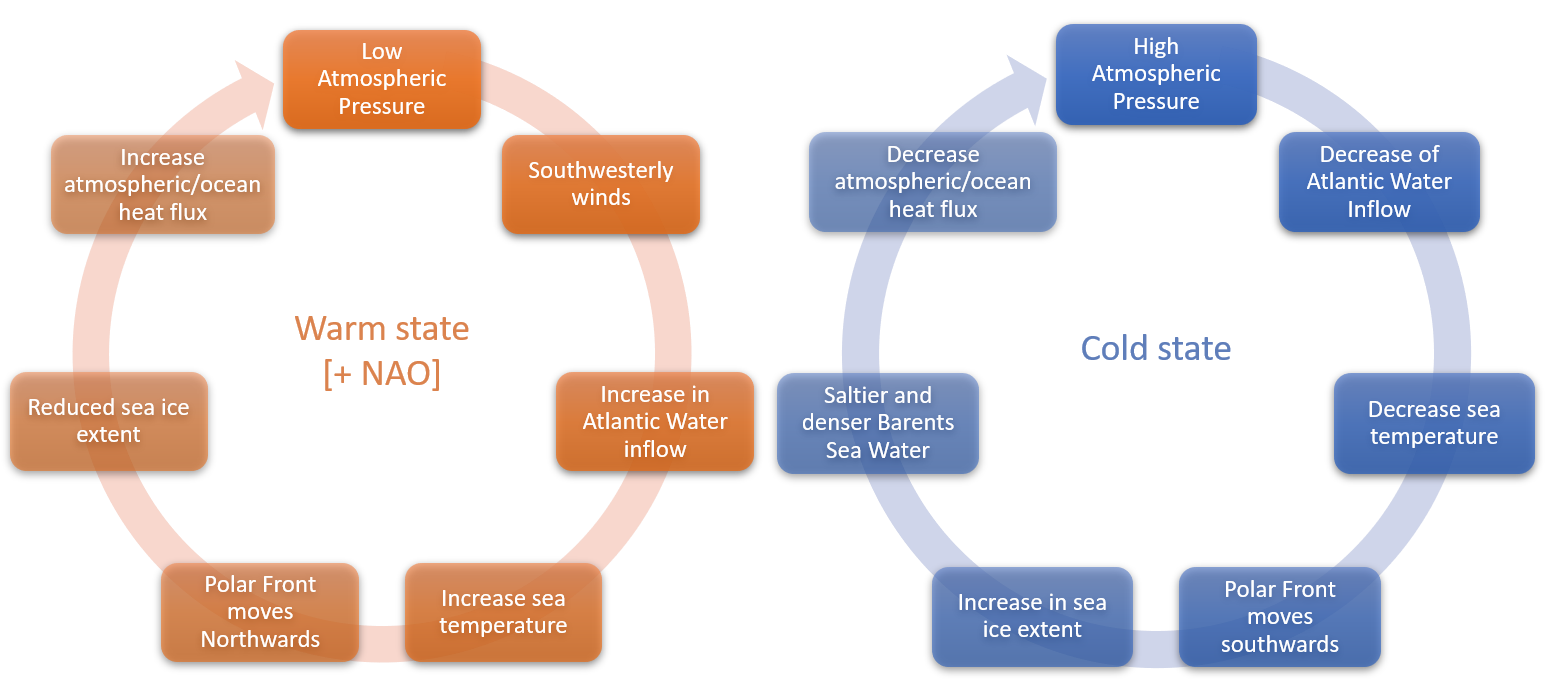
\includegraphics[width=\textwidth]{BSfeedbackloops.png}
	\caption{The warm state (orange), sometimes associated with a positive NAO, is associated with Atlantification of the Barents Sea. The cold state (blue) is associated with more brine, therefore saltier and denser Barents Sea Water formation which contributes to Arctic Intermediate Water.}
	\label{fig:feedback}
\end{figure}


The cold state stems from high pressure at the Atlantic Water entrance, a reduced Atlantic Water inflow, more sea ice extent and less atmosphere/ocean heat flux, as described in Figure \ref{fig:feedback}. The NAO is not always indicative of the state of the Barents Sea because some years local winds, bottom water formation or tidal mixing have a stronger impact on the system. Both feedback loops have impacts throughout the Barents Sea and in the Arctic.\\

The annual mean heat inflow into the Arctic is largely driven by warm Atlantic Water entering from the Fram Strait and the Barents Sea Opening \cite{Serreze2007}. Since the 1960's the water mass distribution in the Nordic Seas has changed. The shift in the water mass distribution is largely due to the positive NAO years \cite{Skagseth2008}. In the Barents Sea, the area covered by Atlantic Water has doubled. The positive trend in Atlantic heat input is also called \textit{atlantification} \cite{Aarthun2012}. The last three decades have seen a retreat of 240 km of the ice edge in the eastern Barents Sea \cite{Aarthun2012}. Even though the reduced sea ice cover is more of a local reduction in ice formation rather than a melting of multiyear ice, these trends directly impact the total oceanic sensible heat transport to the Arctic through the formation of Barents Sea Water \cite{Aarthun2012}. In addition to the reduction in sea ice cover in the Barents Sea, \textit{atlantification} affects the Arctic through the weakening of the stratification of the Atlantic Water which facilitates upwards Atlantic Water fluxes and reduces sea ice cover up to the Eurasian Basin \cite{Polyakov2017}\\

In the section below, I will explore the impacts of the variations in the physical oceanography of the Barents Sea on parts of the marine ecosystem.


\section{Barents Sea: A biological perspective}
Water mass variability and sea ice loss are drivers of marine ecosystem dynamics because they affect productivity and species interaction. Atlantification and the warming of the Arctic are especially crucial in the Barents Sea where temperature and seasonality constrain productivity \cite{Post2013}. The abiotic environment is highly variable because of the local and inter-annual changes in winds and climate. The spring bloom timing and position is challenging to study and predict because it is dependent on a highly variable system \cite{Hansen1990}. This section provides an overview of the impact of physical changes on the pelagic ecosystem of the Barents Sea.\\

\subsection{Primary Production}
The spring bloom in the Barents Sea is highly variable and can be unpredictable from year to year. Three factors drive the spring bloom timing: stratification, latitude and irradiance. As the water column stabilizes after being well mixed throughout the winter, stratification allows the nutrients to be available within the upper 20 m. This is an especially important factor along the ice edge where the bloom can be triggered by melt induced stabilization as early as mid-April \cite{Skjoldal1987}. The other two factors, latitude and irradiance, are closely related. Unlike stratification and irradiance, latitude as a spring bloom factor is predictable. Latitude is a proxy for determining the duration of daylight for an area given the date. Higher latitudes that have the same stratification as a lower latitude will have a later bloom. Irradiance in this context relates to cloud cover, with 30\% clear skies, the earliest possible bloom at the polar front is mid-April \cite{Sakshaug2009}. \\

Even though the seasonal ice edge is prone to an earlier bloom because of the melt induced stratification, the stratified layer only reaches $\sim$ 20 m. It doesn't easily get replenished with nutrients because of the strong pycnocline formed by the freshwater layer from the meltwater. Whereas in ice-free waters, the spring bloom begins much later, in May or June, but can reach 4 to 5 times more biomass because the weaker pycnocline and deeper stratified layer, $\sim$ 50 m, allows nutrients to be replenished with every strong storm \cite{Reigstad2002, Sakshaug2009}. The local reduction in seasonal ice cover will impact primary production and spring bloom timing. In the northern Barents Sea, ice-rich years primary productivity can be 30\% lower than in ice-poor years and ice-free waters tend to have a later bloom \cite{Sakshaug2009}. Arrigo et al. (2008) use a primary productivity algorithm to show that through a progressive loss of sea ice there is an increase in pan-Arctic phytoplankton chl a biomass despite the complex and varied response by each biogeographic region \cite{Arrigo2008, Ardyna2011}. However, the response of increased primary production by lower trophic levels will vary based on changes in stratification, irradiance and nutrient availability \cite{Tremblay2012}. The Barents Sea has a relatively weak stratification which facilitates vertical mixing and upwelling of nutrient rich waters, this suggests that the increase in phytoplankton chl a biomass will be more significant in this eutrophic region \cite{Ardyna2011}.


\subsection{Mesozooplankton}
Copepods dominate the mesozooplankton biomass in the Barents Sea. Among the copepods, there are three abundant \textit{Calanus} species in the Barents Sea. They have different distributions which coincide with the prominent water masses, Atlantic and Arctic, and are adapted to their particular phytoplankton spring bloom conditions. In the Arctic Water, north of the polar front, where the bloom follows the receding seasonal ice edge, \textit{Calanus glacialis} can feed on the intense annual local phytoplankton burst twice throughout its 2-year life cycle \cite{Rey1987, Sakshaug2009}. \textit{Calanus hyperboreus} is also found in the Arctic Water. It is the largest copepod, but it is much less abundant, and the least studied. The intense single bloom in the Arctic Water would not match the 1-year life cycle of \textit{Calanus finmarchicus}. The Atlantic Water, south of the polar front, is a better match for the life cycle of \textit{Calanus finmarchicus} because the bloom is later in the year and longer lasting because of the frequent vertical mixing across the pycnocline.

\subsection{Polar Cod}
Polar cod plays an essential role in the arctic marine ecosystem because it is responsible for most of the energy transfer from zooplankton to top predators \cite{Welch1992}, yet little is known about its population and spatial structure.  Spawning takes place between December and March in two main areas of the Barents Sea. The spawning sites are split between the south-east, the Pechora Sea and along the west coast of Novaya Zemlya, and the west, off the east and west coast of Svalbard. The most abundant and most variable spawning area is the Pechora Sea. Also, the relative abundance is variable between eastern and western spawning sites \cite{Eriksen2015}. Variability in distribution and abundance of polar cod in the Barents Sea is expected to increase as the survival of eggs and larvae are closely correlated to the balance between sea ice extent and Atlantic Water inflow \cite{Hop2013, Eriksen2019, Huserbraaten2019}. \\

Eriksen et al. (2019) define polar cod spawning habitat suitability using four criteria: ice cover for egg protection and light availability for larval feeding, match/mismatch hatching with plankton bloom timing for prey availability, thermal incubation requirements of eggs, and thermal growth requirements of larvae. In the Canadian Arctic, studies hypothesize polar cod survival is positively correlated with earlier hatching in the freshwater from meltwater in the spring \cite{Bouchard2011, Bouchard2015, Bouchard2017}. The conflicting polar cod larvae survival hypotheses are unsure whether maximizing pre-wintering size by early hatching (freshwater winter refuge hypothesis) \cite{Bouchard2017} or ensuring essential prey abundance through later hatching coinciding hatching with local zooplankton bloom production (match/mismatch hypothesis) \cite{Cushing1994, Eriksen2019} is most important for survival.\\

The polar front creates a biogeographical transition zone between boreal and arctic ecosystems \cite{Eriksen2015}. It is difficult to survey because of vessel costs and ice edge proximity during the winter and spring. For my thesis, I will use cutting edge surveying methods and acoustic instruments to improve our understanding of the epipelagic ecosystem in the Barents Sea.





\section{Context of Study}
\subsection{Main research question}
The overarching goal of this thesis is to \textbf{improve the monitoring the epipelagic layer with ASVs equipped broadband echosounders to increase our understanding of the epipelagic ecosystem}. In the sections below I outline the three proposed chapters of my thesis.

	
\section{Chapter 1: Spatial and vertical distribution of zooplankton near the surface from Sailbuoy deployments}

\subsection{Context}
In the Barents Sea, the Svalbard branch of the West Spitsbergen Current (Atlantic Water inflow) advects warm salty water containing zooplankton and fish species of boreal origins in Whalers Bay north of Svalbard (Figure \ref{fig:whalers}) \cite{Falk-Petersen2015}. Based on seabirds and marine mammals feeding on the surface waters and satellite observations of ocean surface colour \cite{Basedow2019}, the Atlantic Water inflow upwelling north of Svalbard is expected to have high biological activity. In Tromsøflaket (Figure \ref{fig:whalers}), zooplankton and cod larvae have only been determined by net samples and hull-mounted echosounders. These traditional sampling methods do not preserve the natural vertical distribution or identify the species throughout the surface of the water column. 


\begin{figure}[H]
	\centering
	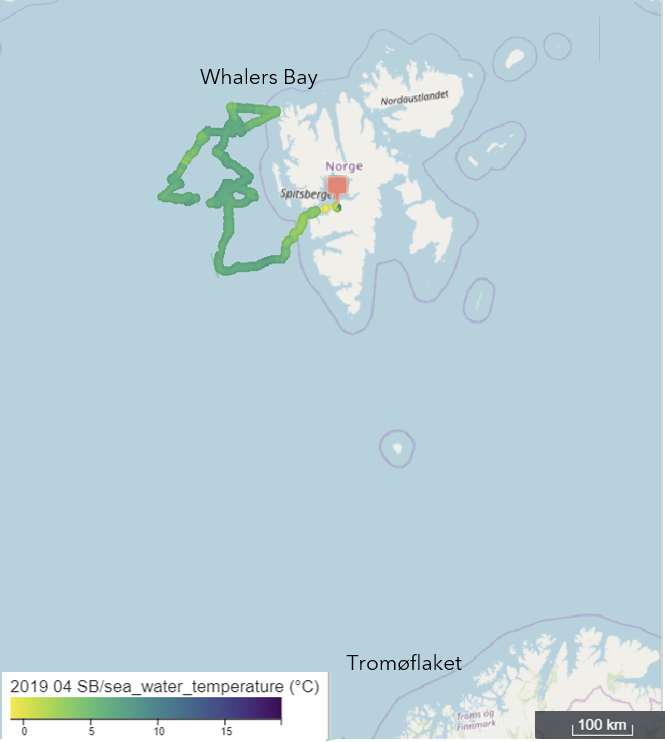
\includegraphics[width=0.6\textwidth]{SB2019WhalersBay.png}
	\caption{The trajectory of the Sailbuoy survey in Whalers Bay from August 13th 2019 to September 27th 2019. The colour of the trajectory represents the sea surface temperature. Tromsøflaket is just off the coast of Northern mainland Norway.}
	\label{fig:whalers}
\end{figure}

\subsection{Genereal Objective}
Conventional hull-mounted acoustic surveys show little biological activity in the upper 200 m in Whalers Bay but remote sensing has shown detection of a epipelagic active layer of copepods near the surface. The effect of the blind zone of hull-mounted echosounder and vessel avoidance from survey ships in the epipelagic layer needs to be quantified for accurate spatial and vertical estimates of distribution of zooplankton. Saibuoys provide an opportunity to increase spatial and temporal coverage while surveying without light and noise pollution. I will compare of the vertical distribution of the active layer in Tromsøflaket and Svalbard from Sailbuoy broadband echosounder data to compare the epipelagic active layer in a southern coastal region and an Arctic region.

\subsection{Research Questions}
\begin{itemize}
	\item{Where is the active layer in Tromsøflaket and what is it composed of?}
	\item{What are the benefits and drawbacks of autonomous surface vehicles as a survey platform?}
	\item{What differences and similarity between the active layer Tromsøflaket and Svalbard?}
\end{itemize}

\subsection{Specific Objectives}
\begin{itemize}
	\item{Assess the vertical distribution of cod larvae and \textit{Calanus} in Tromsøflaket;}
	\item{Identify differences in results from boat mounted acoustic surveys and Sailbuoy surveys;}
	\item{Compare the active layer within Tromsøflaket and with Whalers Bay.}
\end{itemize}

\subsection{Methods}
\subsubsection {Zooplankton Distribution}
Analyze Tromsøflaket Sailbuoy survey data from the 2018 deployment for zooplankton distribution. Use the complimentary tows and vessel data to validate and contextualize and identify layers, presence/absence and trends in the Tromsøflaket Sailbuoy data.

\begin{figure}[H]
	\centering
	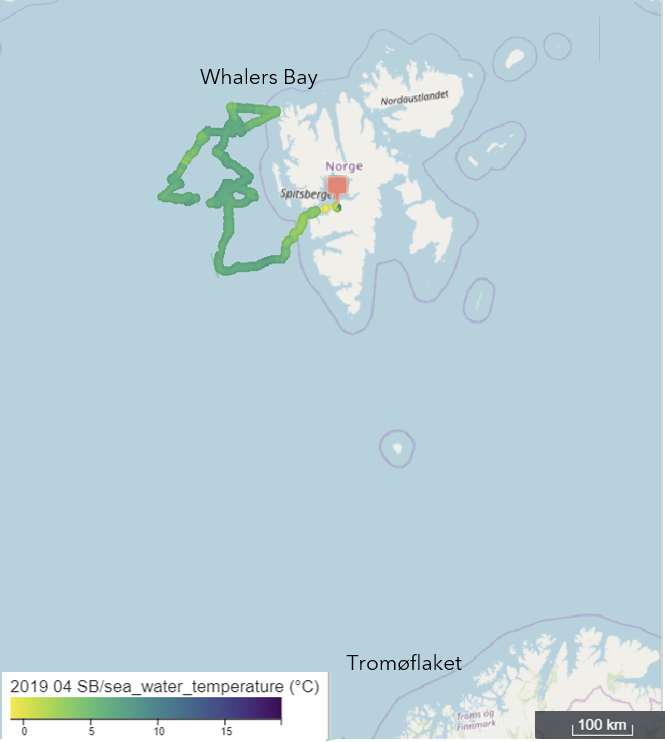
\includegraphics[width=0.6\textwidth]{SB2019WhalersBay.png}
	\caption{The trajectory of the Sailbuoy survey in Whalers Bay from August 13th 2019 to September 27th 2019. The colour of the trajectory represents the sea surface temperature. Tromsøflaket is just off the coast of Northern mainland Norway.}
	\label{fig:whalers}
\end{figure}
 
\subsubsection {Boat mounted surveys and Sailbuoy surveys}
I will then create a temporal and spatial abundance map of zooplankton distribution from the Sailbuoy data. I will also create a temporal and spatial abundance map of zooplankton distribution from the vessel mounted acoustics dataset. I want to quantify and describe the differences while highlighting the bias, benefits and the limitations of each survey method.

\subsubsection {Active layer comparison}
I will use the available Sailbuoy survey data from Tromsøflaket 2018 and Svalbard 2019 for a comparison of the the epipelagic active layer in a southern and coastal region and an Arctic region. I will compare their composition, center of mass, maximum backscattering strength, thickness and occurrence.





\section{Chapter 2: Acoustic signature of dominant Arctic species from a microcosm experiment}
\subsection{Context}
A Sailbuoy equipped with broadband echosounder offers increased spatial and temporal resolution and acoustic target classification \cite{Korneliussen2018} at a lower cost than boat surveys. The broadband echosounder collects continuous measurements of frequency-dependent backscatter \cite{Bassett2017}; but the resulting datasets are too large for traditional processing methods. Traditional methods for processing echosounder data are time-consuming, introduce biases and are irreproducible. Data management and processing methods for ocean surveys have fallen behind on the technology advancements. Though developments in broadband echosounders have the potential to increase taxonomic resolution, Basset et al. (2017) states that species identification using broadband will face the same challenges as narrowband at similar frequencies, but he also concludes that “The challenges of working with broadband systems will be reduced as the technology is more widely adopted and new processing techniques are developed to identify and exploit the additional information inherent in broadband signals” \cite{Bassett2017}. \\

Broadband echosounder measurements are favored in high-latitudes where backscatter is dominated by a single species \cite{DeRobertis2019}. The epipelagic layer of the Barents Sea has few prominent species. This characteristic makes it an ideal region to develop classification methods and tools because there are fewer species to differentiate.

\subsection{General Objective}
Characterize the acoustic signal of species that dominate in the epipelagic layer of Barents Sea using \textit{ex situ} experiments, \textit{in situ} survey data, and acoustic model results.

\subsection{Research Questions}
\begin{itemize}
\item{What is the modelled frequency response of \textit{Calanus} and polar cod larvae?}
\item{What is the \textit{ex situ} frequency-response curve of \textit{Calanus} and polar cod larvae?}
\item{Can the isolated acoustic signature be used to identify species in \textit{in situ} Sailbuoy survey data?}
\end{itemize}

\subsection{Specific Objectives}
\begin{itemize}
\item{Model the acoustic signature of species using their sound speed and density properties;}
\item{Document the frequency-response curve of species that dominate the epipelagic layer of the Barents Sea;}
\item{Identify the signal in survey vessel mounted and Sailbuoy broadband echosounder data.}
\end{itemize}

\subsection{Methods}
\subsubsection{Acoustic scattering model of targeted species}
Use an approximate acoustic scattering model to study the scattering surface for the range of frequencies available by the 333 kHz broadband echosounder. The scattering surface will be modeled to represent \textit{Calanus} and polar cod larvae. I will have to obtain sound speed and density properties of the targeted species though frozen samples or estimates.

\subsubsection {Build microcosm cage} 
Develop a experimental method for isolating frequency-response curves of monocultures. I will design a net cuboid inside a cage that is big enough to allows the species to moves freely inside but small enough to deploy easily. The WBAT and 333 kHz transducer will be 4 m above the net, the acoustic beam will be ensonifying the species as would the Sailbuoy during a survey. Once the net is built, I will test the acoustics of the frame and net design. I will do measurements of a known target without the cage, such as a calibration sphere, the empty net and the net with a calibration sphere at different locations in the net \cite{Foote1990}. I will deploy the cage in a aquaculture net at Kårvika and populate the net with monocultures of \textit{Calanus} and monocultures of polar cod larvae. I will use 333 kHz (and 200 kHz) transducers with the WBAT to collect many detections of freely swimming species within the net.

\subsubsection {Identify each species acoustic signature probability function} 
I will identify the signature of \textit{Calanus} and polar cod larvae in Sailbuoy survey data. All the isolated targets will be combined to create a probability function for each species. I will use a recent study in assessments of broadband echosounder data processing effects to improve the classification and identification methods \cite{BenoitBird2020} and compare to our results for window length of the Fourier transform, frequency bandwidth and position of targets in the beam. I will use the frequency response probability functions in hull-mounted and Sailbuoy mounted survey data.




\section{Chapter 3: Describe the distribution of age-0 polar cod across the polar front in the Barents Sea}
\subsection{Context}
In the Canadian Arctic, recruitment estimates for the adult population of polar cod (\textit{Boreogadus saida}) use the abundance of epipelagic, age-0 polar cod as a predictor. Abundance estimates from Canadian Arctic seas (2012-2017) are calculated from hull-mounted acoustic surveys \cite{Bouchard2017, LeBlanc2019}. Age-0 polar cod in the blind zone, 2 - 13 m, are excluded from biomass recruitment estimates.  \cite{Bouchard2016} has documented the vertical distribution of polar cod in the Beauford Sea and found that 59\% of the population were within 10 m from the surface between June and August. \\

In this chapter, I will use the Sailbuoys reduced blind zone to improve the resolution of polar cod larvae vertical distribution in epipelagic layer of the Barents Sea. ASVs equipped with broadband echosounders are especially valuable when deployed over long periods in remote areas that are difficult or expensive to access with conventional boat methods, which is the case for Baffin Bay in the Canadian Arctic and the polar front in the Barents Sea.

\subsection{General Objective}
ASVs could improve recruitment estimates of polar cod in the Barents Sea.  I will use Sailbuoys to quantify the abundance of age-0 cod in the Barents Sea, specifically across the polar front. I will compare with the results from a coincident boat mounted survey with narrowbeam echosounders to quantify the missing age-0 cod in the blind zone and compare methods.

\subsection{Research Questions}
\begin{itemize}
	\item{Where are the polar cod larvae relative to the polar front? }
	\item{Can we extrapolate or replace vessel mounted narrowband multi-frequency analysis with trawls surveys to broadband echosounders on ASVs with a great spatial coverage;}
	\item{What is their vertical structure? Are they at the surface in the fresher surface water, throughout the mixed layer or the entire water column?}
\end{itemize}

\subsection{Specific Objectives}
\begin{itemize}
	\item{Assess the distribution of polar cod larvae on both sides and across of the polar front;}
	\item{Compare multifrequency analysis from vessel mounted narrowband 70 and 120 kHz compare to broadband 333 kHz species identification analysis;}
	\item{Use the reduced blind zone of the Sailbuoy to quantify abundance in the epipelagic layer of the Barents Sea.}
\end{itemize}

\subsection{Methods}
\subsubsection {Multi-platform sampling plan}
The R.V Helmer Hanssen is going to the polar front in May 2021 for a research cruise. I will design a sampling plan for surface and underwater gliders, vessel acoustics, ichthyoplankton net sampling and UVP6 sampling across the polar front. The sampling plan will be designed to maximize the crossing of the polar front to quantify the gradient of change in ecosystem from an Atlantic Water dominated region to a purely Arctic Water region.

\subsubsection {Multi frequency analysis}
I will use the difference in mean volume backscattering strength to set thresholds for classification of target categories \cite{Bouchard2017, LeBlanc2019}. Then, I can identify signals from polar cod larvae from zooplankton swarms. I will compare the multi-frequency analysis results to species identification from broadband echosounders from the isolated acoustic signatures in Chapter 2.

\subsubsection {Fine scale vertical resolution}
Use the high resolution data of an undisturbed epipelagic layer to study the vertical structure of species that dominate the Barents Sea at the polar front.


\section{Timeline}

\begin{figure}[H]
	\centering
	\includegraphics[width=\textwidth]{timeline.png}
\end{figure}




\addcontentsline{toc}{section}{References}
\bibliography{BiblioProp}
\bibliographystyle{apalike}


\end{document}